\section{Problem Definition} \label{sec:problem-definition}

The rapid advancement of artificial intelligence and machine learning techniques has paved the way for transformative developments in content creation across multiple disciplines. However, a significant gap remains in the field of audio synthesis, especially in the context of generative \ac{AI} models. The challenge at hand is to bridge this gap and enable the transformation of textual input into high-fidelity and immersive soundscapes, thereby creating a new form of creative expression.

Recently, the landscape of audio generation has been undergoing a paradigm shift, catalyzed by significant investments and efforts from prominent technology conglomerates. As of 2023, major industry players are placing significant bets on the potential of \ac{AI}-driven audio synthesis. This noteworthy development underscores the growing recognition of the transformative impact that sophisticated audio generation can have across sectors, including entertainment, education, virtual reality, and more.

\subsection{Gap in the Literature}

The landscape of audio synthesis through generative \ac{AI} models presents a spectrum of challenges and limitations that impact various applications, including content creation, sound design, music production, and interactive media. These challenges include computational constraints, model architectural intricacies, quality/realism trade-offs, data-related hurdles, interpretability issues, and scalability concerns. Addressing these limitations has the potential to significantly improve the quality and utility of audio synthesis methods.

Significant hurdles in the use of generative \ac{AI} models for audio synthesis are the computational cost and the training time. PixelCNN Decoders~\cite{oord_conditional_2016}, Jukebox~\cite{dhariwal_jukebox_2020}, and Hi-Fi GAN~\cite{kong_hifi-gan_2020}, which exemplify these models, require extensive computational resources and long training times. These limitations render these models inaccessible to researchers and developers and limit their applicability in real-world situations where efficient generation is critical. Developing more efficient training algorithms or model architectures could democratize access and broaden the reach of audio synthesis methods by overcoming these challenges.

Producing \textbf{high-quality and realistic audio} synthesis is a complex task. The lack of ability to capture minute details, as seen in models such as WaveNet~\cite{oord_wavenet_2016} and MelGAN~\cite{kumar_melgan_2019}, causes audio outputs to be deficient in delicate nuances and textures. Limitations such as mode collapse, seen in GANSynth~\cite{engel_gansynth_2019}, and Jukebox~\cite{dhariwal_jukebox_2020} can cause a lack of variety, leading to repetitive and monotonous audio outputs. Additionally, maintaining coherence throughout extended audio sequences - as observed in PixelCNN~\cite{oord_conditional_2016}, WaveNet~\cite{oord_wavenet_2016}, Jukebox~\cite{dhariwal_jukebox_2020}, and Riffusion~\cite{forsgren_riffusion_2022} - is a challenge that can affect the final output.

The versatility of synthesis models is impacted by data efficiency and generalization capabilities. Models such as DALL-E~\cite{ramesh_zero-shot_2021}, VALL-E~\cite{wang_neural_2023}, and MusicLM~\cite{agostinelli_musiclm_2023} have suboptimal data efficiency, which requires large datasets for effective training. It is crucial to address the challenges in handling unusual concepts, as observed in \ac{GLIDE}~\cite{nichol_glide_2021}, to broaden the creative potential of these models. Moreover, the practical utility and user-friendliness of models such as DALL-E~\cite{ramesh_zero-shot_2021} and VALL-E~\cite{wang_neural_2023} are constrained due to their limited control and interpretability.

The challenges and limitations within audio synthesis through generative \ac{AI} models align with the key objectives of this thesis. The aim to develop advanced systems that handle sound, classification, and end-to-end generation while accounting for hardware limitations aligns with the need to overcome computational constraints highlighted in the literature. The thesis aims to address the computational hurdles that hinder the accessibility and practicality of audio synthesis models by devising more efficient training algorithms or model architectures. This directly contributes to the broader objective of providing valuable contributions to deep learning and its applications.

The goal to create end-to-end systems that generate sound from any textual input is intricately connected to the challenges of quality, realism, and coherence in audio synthesis. The thesis aims to bridge the gap between textual input and high-fidelity, immersive soundscapes by exploring the intricacies of model architectural design and refining the generation process. Evaluating the accuracy of generated audio aligns with the broader pursuit of overcoming limitations in capturing fine-grained details, mode collapse, and long-term coherence. This pursuit ultimately enhances the authenticity and richness of the synthesized audio.

The ambitious mission to contribute to \ac{DL} and its applications aligns well with the goal of addressing data-related issues, such as biases and limitations arising from training data. This thesis aims to enhance the adaptability of generative \ac{AI} models by curating diverse and representative datasets and implementing techniques for bias detection and mitigation, to make them more responsive to various tasks and domains. This alignment highlights the research's importance in advancing audio synthesis and establishing a wider framework for responsible and inclusive development of \ac{AI}.

To summarize, the literature's identified gap, marked by challenges ranging from computational constraints and quality/realism to data efficiency and interpretability issues, is intricately linked with this thesis's objectives. Advancing end-to-end audio synthesis systems while addressing these challenges not only deepens the field's scientific comprehension but also profoundly aligns with the broader goals of your research endeavor.

\subsection{Formal Problem Definition}

The goal of this study is to address the synthesis of audio based on textual prompts. The audio is not limited to a specific domain, such as speech or music. The audio produced by the model must be dependent on the inserted textual input. The generated audio must be produced in real-time, with minimal latency after the textual prompt is inserted into the model. This study considers a model that resolves this issue and refers to it as an end-to-end model. Furthermore, it is considered that the terms end-to-end and text-to-sound are interchangeable in this context.

These models are trained using sounds labeled by humans from openly available datasets. Furthermore, the evaluation involves comparing the generated sounds with their corresponding real sounds.

To formally define this problem, the elements in Figure~\ref{fig:problem-definition} must be defined.

\begin{figure}[ht]
    \centering
    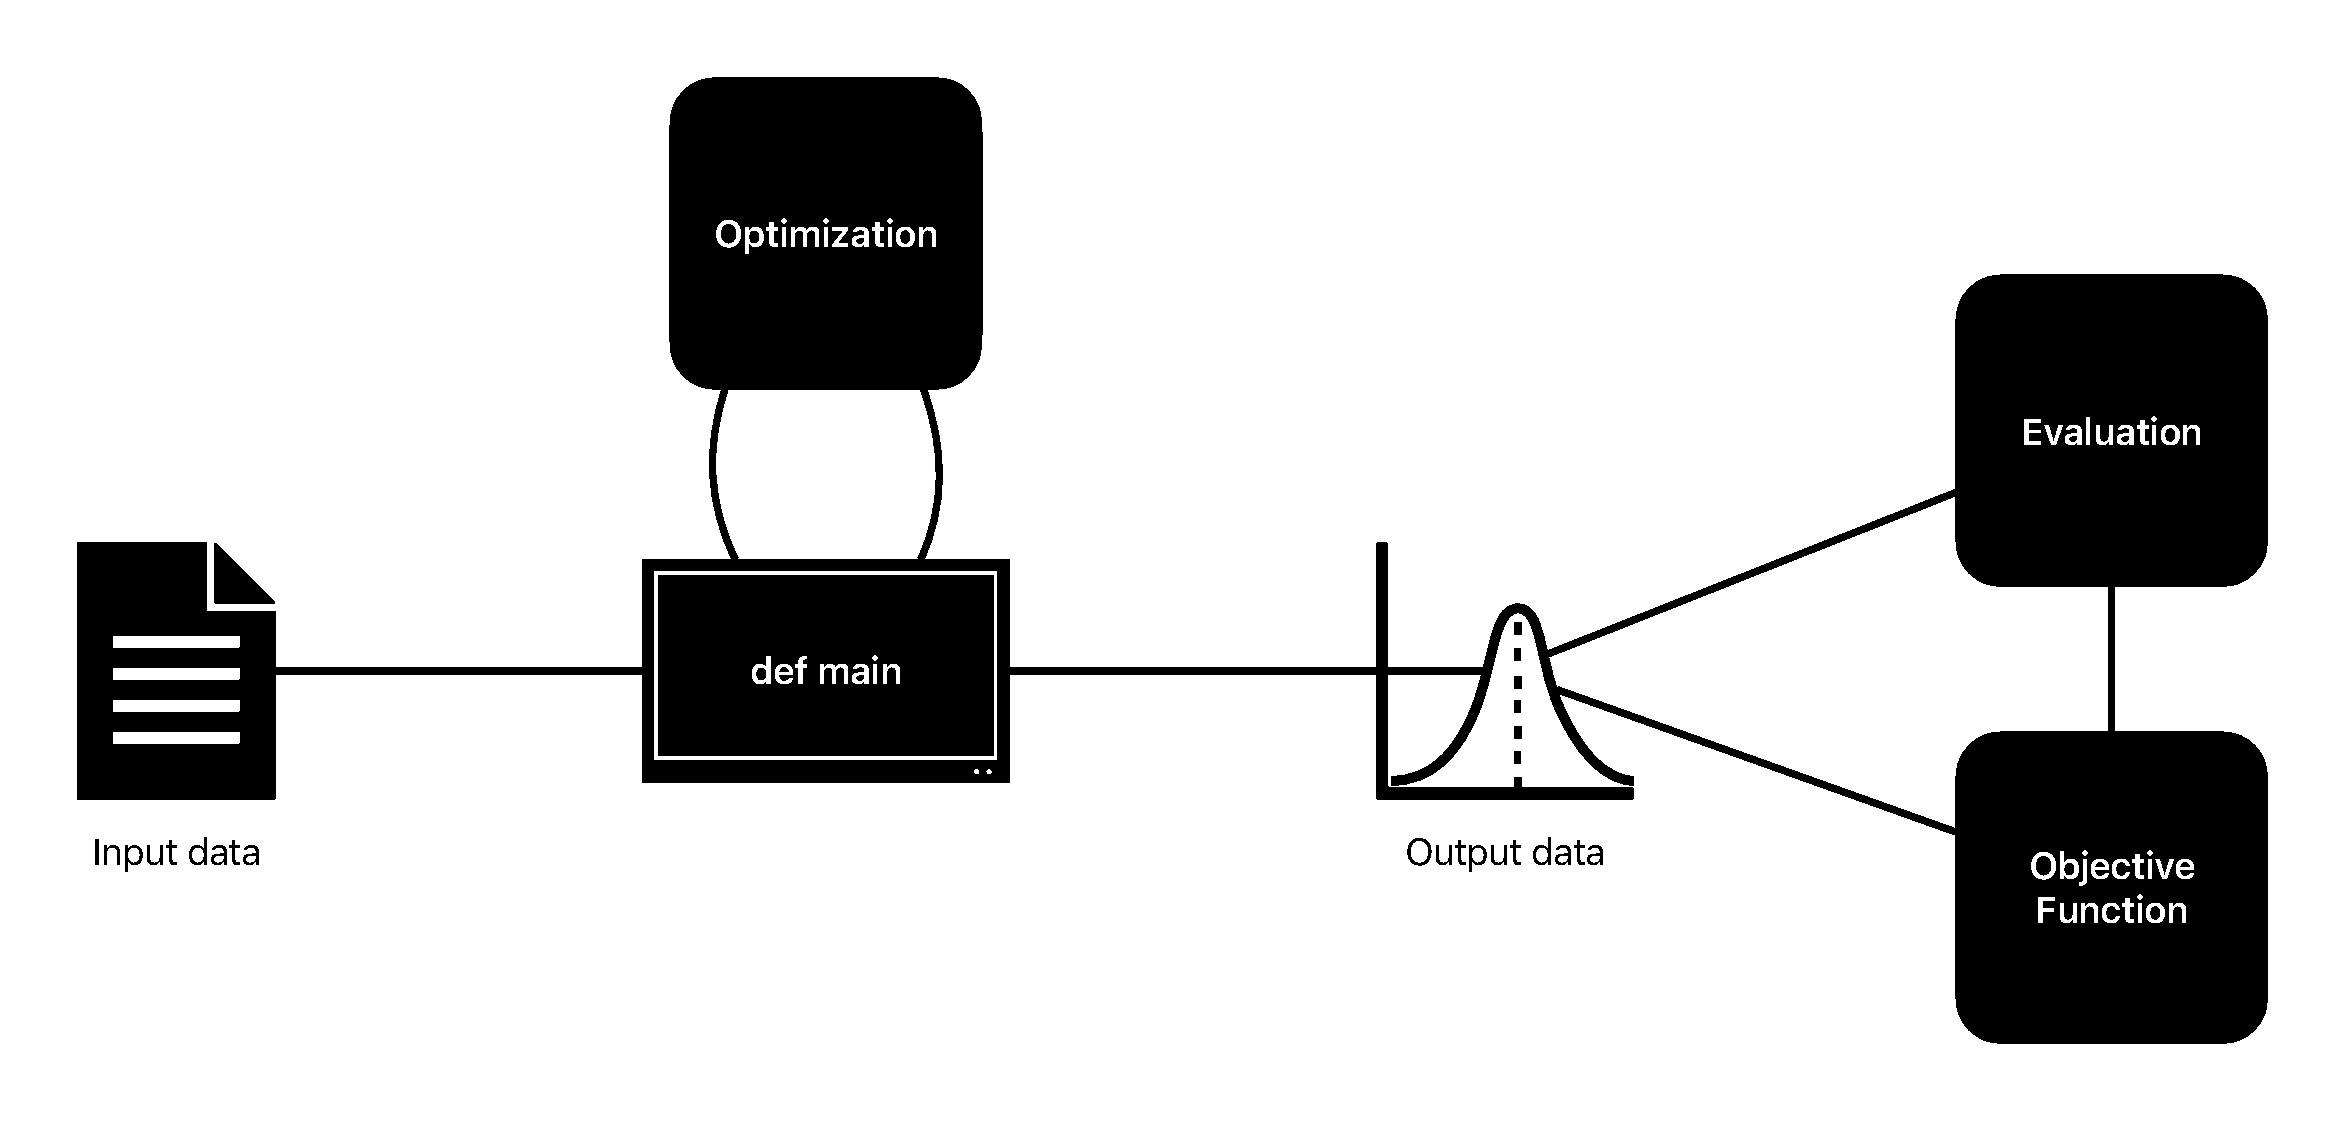
\includegraphics[width=\textwidth]{figures/3-problem/Problem-Definition.pdf}
    \caption{AI Problem Definition}
    \label{fig:problem-definition}
\end{figure}

\subsubsection{Input Data}

Synthesizing audio from textual prompts entails several challenges, especially when dealing with the diverse formats present in sound samples and text labels. As these formats converge, they add layers of intricacy that require innovative solutions and thoughtful consideration.

In the audio domain, dealing with diverse formats manifests itself in multiple sonic expressions, ranging from music and spoken dialogues to environmental noises and abstract compositions. These formats encompass a spectrum of acoustic textures and temporal dynamics, demanding a unique processing and analysis approach for each.

Text labels also introduce a variety of challenges as they take various forms from different sources. The range of text labels spans from brief categorical tags that capture high-level features to verbose textual descriptions that explore intricate details. This variation poses the model with the task of decoding and utilizing the diverse meanings, tones, and contexts embedded within these labels. Achieving balance between the weight of these different formats while incorporating them into the generative fabric poses its own challenge.

The intersection of different audio formats and textual labeling structures presents a challenge for the model to generate coherent and harmonious audio outputs. Each format has its implicit dimensions, nuances, and potential biases associated with it. Ensuring that the model avoids being biased towards a particular format or ignores others is a challenge that needs precise calibration. Additionally, the model must handle the complex task of cross-modal learning, deciphering the interplay between sound and text to produce outputs that match seamlessly with textual prompts.

When embarking on the complex process of audio synthesis from text, it is important to acknowledge the intricacies that arise from combining sound samples and text labels. The difficulties that come with handling various formats serve as milestones of progress and discovery. These challenges put the model's true capabilities to the test as it navigates through the maze of formats, becoming a creative force capable of orchestrating sonic symphonies that blend seamlessly with the tapestry of human expression.

\subsubsection{Output Data}

The output produced by these models is in a particular audio format, resulting from the complex interplay between textual cues and sonic expression. An essential factor in this synthesis is real-time generation, which is critical for both user experience and practical applications.

Real-time generation has the potential to provide immediate results, smoothly converting textual input into audio output. In practical contexts, such as interactive media, virtual environments, or assistive technologies, the capability to respond promptly to user inputs with sonic output enhances the immersive quality of the experience.

The pursuit of real-time generation comes with its share of difficulties and trade-offs. The requirement for swift responsiveness can create limitations that may affect the precision and complexity of the produced audio. The delicate balance between speed and sonic complexity requires careful consideration.

Real-time generation plays a critical role in generative audio synthesis. Achieving real-time outputs requires a balance between immediacy and auditory finesse, guided by studies on human perception. During this pursuit, the generative model attunes itself not only to the cadence of textual cues, but also to the rhythm of human interaction and appreciation.

\subsubsection{Objective Function}

The development of an objective function is a crucial step in this work, where challenges, strategies, and insights come together to shape the core of creative synthesis.

The purpose of generative models is to uncover and encapsulate the complex distributions that form the basis of the data. This journey of comprehension accompanies the aspiration to create new data, which evokes familiarity with the original while testing the limits of artistic innovation. This essence, charming as it may be, emerges within a paradox that challenges us to bridge the gap between accuracy and realism by channeling the learned distributions into outputs that reflect authenticity.

The challenge in defining an objective function lies in extracting the core components of accuracy and realism, and quantifying them into a measurable metric. One approach that aligns with the generative pursuit involves reducing the divergence between the original and synthesized data.

Within the realm of generative literature, numerous strategies intertwine to inspire the creation of objective functions. Approaches presented in Section~\ref{sec:evaluation} should be taken into account.

The objective function emerges as a guiding principle in this interplay of creativity and computation. The objective function embodies the urge for realism and accuracy, reflecting the very essence of generative models in its mathematical grasp. The definition of the objective function is intertwined with the fabric of the generative narrative, uniting aspirations and strategies into a symphony that echoes across the domains of imagination and reality.

\subsubsection{Optimization Algorithm}

The optimization algorithm aims to shape the generative landscape based on the objectives defined within the objective function.

Selecting an optimization algorithm is a crucial decision in this field that needs careful consideration. Each generative model has its own intrinsic characteristics, strengths, and idiosyncrasies, and it is these traits that determine the choice of optimization algorithm. The algorithm guides the process towards optimal solutions and shapes the generative narrative with each iterative step.

Selecting an optimization algorithm is an arbitrated process where the properties of the generative model are tailored to the unique contours of problem landscape. It entails a delicate calibration to adapt the nuances of established algorithms, harmonizing them with the demands of the generative journey. Fine-tuning hyperparameters, sculpting convergence criteria, and managing trade-offs are integral facets of optimization.

The optimization landscape within the explored generative models consists of various algorithms that align with the specific requirements of each model.

Exploring optimization algorithms reveals a landscape that mirrors the fusion of disciplines within generative fields. Gaining insights from seminal works across various optimization methodologies, the optimization algorithm acts as a creative tool, ready to enhance the generative canvas with precision and convergence.

\subsubsection{Evaluation Metrics}

Evaluation metrics are necessary to guide exploration into the realm of generative models.

However, evaluating generative models involves navigating uncharted territories, especially when considering the intricate realm of subjective attributes. The concepts of audio realism, coherence, and emotive resonance are subjective, making it challenging to measure them objectively. Achieving sound realism requires balancing the timbral fidelity and temporal authenticity, which creates a challenge requiring innovative solutions. Similarly, coherence in generative outputs, determined by the harmony among sequential elements, necessitates metrics that can reveal the intricate patterns.

Specific evaluation metrics emerge in this pursuit as guiding stars, each one poised to illuminate a unique facet of generative prowess. Perceptual audio quality metrics, which are rooted in the perceptual space of human hearing, transcend the realm of raw signal processing. They reflect the intricate tapestry of auditory perception. Subjective metrics such as \ac{MOS} are used. Research delves into the visceral nature of human judgment and provides a medium on which subjective impressions are recorded.

Among the many metrics, their relevance, appropriateness, and coherence with the generative narrative are crucial. Metrics anchor the ephemeral expanse of creativity to the solid ground of quantitative analysis.